% !TeX root = ./jvk-blatt1.tex

\excercise{Task und UI}
\label{ex5}

\begin{enumerate}
    \item Nun wollen wir in der Main Klasse, durch
    den \lstinline{Sheet1Task5} wie hier gezeigt ein Spiel starten:
    
    \begin{lstlisting}
    Game demoGame = new Game("Hello World", new Sheet1Task5());
    \end{lstlisting}
    
    Du startest das Spiel in der Variable \lstinline{demoGame} indem du die Operation \lstinline{run()} darauf aufrufst.
    
    \begin{lstlisting}
    demoGame.run();
    \end{lstlisting}
    
    Starte das Programm in IntelliJ, mit dem kleinen Play-Button oben in der Werkzeugleiste und schau dich ein wenig im Fenster, welches aufgeht um.
    
    \vspace{5mm}
    
    \item In der vorherigen Teilaufgabe hattest du bereits ''Hello World'' und ein Task-Objekt an Game übergeben.
    Nun wollen wir noch ein TaskVerifier-Objekt übergeben.\\
    Orientiere dich dazu am unteren Bild. Starte, nachdem du fertig bist, das Spielfenster neu. \\
    
    Was verändert sich im Spielfenster?
    Finde den \q{Task Status} Tab und drücke den Refresh Button.
    
    \begin{lstlisting}
    Game demoGame = new Game("Hello World", new Sheet1Task5(), new Sheet1Task5Verifier());
    \end{lstlisting}
    
    \end{enumerate}

    \begin{enumerate}\setcounter{enumi}{2}

        \item Finde sowohl im Spiel als auch in IntelliJ die Konsole. Dies ist ein Feld in dem Text ausgegeben wird:
        \begin{center}
        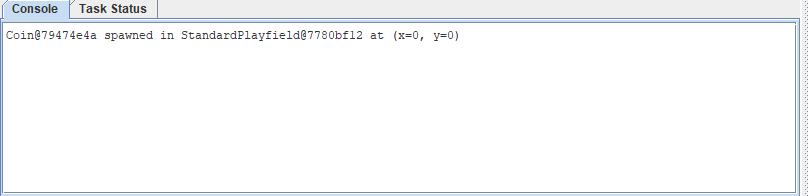
\includegraphics[width=\linewidth]{./figures/console.PNG}
        \end{center}
        
        In der Konsole siehst du, dass eine \texttt{Nut}(Nuss) gespawnt  wurde.
        Finde die Koordinaten des Feldes, auf welchem die \texttt{Nut} gespawnt wurde.
        
        \item Nun suche nach der Stelle im Code in der Klasse \lstinline{Sheet1Task5}, in dem die erste Nuss erzeugt wird.\\
        Hinweis: \lstinline{Sheet1Task5} findest du im \lstinline{project/src/main/java/de/unistuttgart/informaitk/fius/jvk/tasks}-Ordner des Projektes.
        \newpage
        \item Nun wollen wir endlich mal selber Nüsse auf das Spielfeld platzieren.
        Hierfür bearbeitest du die Klasse \lstinline{Sheet1Task5}.\\
        Platziere mindestens 5 Nüsse auf beliebigen Feldern.
        
        Benutze den \q{Task Status}, um herauszufinden, ob du die Aufgabe erfolgreich gelöst hast.
        
        Wie ist der Zusammenhang zwischen Position der Nuss und den Koordinaten im Koordinatensystem?
        
        \textbf{Tipp:} Wenn du nicht genau weißt, wie eine Nut erzeugt wird, schaue dir den Code in Teilaufgabe d) erzeugten Code nochmal an.
        \item Du kannst auch im Fenster selbst Nüsse und Wände platzieren, dies geht rechts oben mit dem + und - Button. Versuche die Aufgabe e) nun nochmal zu lösen, ohne im Code eine Nuss zu platzieren.
        \end{enumerate}
